\chapter{Autómatas}
\section{Autómata Finito Determinístico (AFD)}
\subsection{Definición}
Un Autómata Finito Determinístico (AFD) es una quintupla $M=(k,\Sigma,f,s_0,F)$ donde:
\begin{itemize}
\item $k$ conjunto finito no vacio, \textit{conjunto de estados}
\item $\Sigma$ conjunto finito no vacio, \textit{Alfabeto}
\item $f:k\times\Sigma\rightarrow k$ , \textit{Funcion de transicion}
\item $s_0\in k$, \textit{Estado inicial}
\item $F\subseteq k$, \textit{Conjunto de estados finales}
\end{itemize}
\subsection{Intepretación}
Podemos verlo como una cinta que posee una \textbf{cabeza lectora}, esta se mueve hacia la derecha y con este movimiento los estados $q_i$ cambian.
\begin{figure}[ht!]
\centering
\begin{tikzpicture}

\draw(-3,5) -- (3,5);
\draw(-3,4) -- (3,4);

\newcount\foo
\foo=-3
\loop
  \message{\the\foo}
  \draw(\foo,5) -- (\foo,4);
  \advance \foo 1
\ifnum \foo<4
\repeat

\node[] at (-2.5,4.5) 
    {b};
\node[] at (-1.5,4.5) 
    {b};
\node[] at (-0.5,4.5) 
    {a};
\node[] at (0.5,4.5) 
    {b};
\node[] at (1.5,4.5) 
    {a};
\node[] at (2.5,4.5) 
    {b};

\node[] at (-0.5,5.4) 
    {{\color{red}``\texttt{{\scriptsize Cabeza Lectora}}''} };
\draw[line width=0.4mm, red] (-1.1,3.9) -- (0.1,3.9) -- (0.1,5.1) -- (-1.1,5.1) -- (-1.1,3.9);

\draw[line width=0.2mm](-2,1) -- (2,1) -- (2,3) -- (-2,3) -- (-2,1);
\draw(-5,0.5) -- (5,0.5);

\draw[line width=0.2mm] (-1.5,0.75) circle (7pt);
\draw[line width=0.2mm] ( 1.5,0.75) circle (7pt);

\draw [->,very thick](2,2) -- (3,2);

\newcounter{cA} 
\newcounter{mycounter}
\newcommand\x{0}
\forLoop[45]{0}{8}
{%
  \node[] at ({sin(\i)*0.75},{cos(\i)*0.75+2}) {$q_{\thecA}$};
  \x = \the\numexpr\x+1 \relax;
  \addtocounter{cA}{1};
}
\draw [->,very thick](0,2) -- ({sin(150)*0.5},{cos(150)*0.5+2});

\end{tikzpicture}
\caption{Es importante notar que un Autómata se mueve hacia \textit{adelante} al contrario de una máquina de Turing \texttt{2.9}}
\end{figure}
\pagebreak
\subsection{Representación}
\subsubsection*{Tabla}
En esta representación, el estado inicial se apunta con una \textbf{flecha}($\rightarrow$), los estados finales se \textbf{subrayan}.
\begin{figure}[ht!]
\centering
\begin{tabular}{|c|cccccc|}
    \hline
    \backslashbox{$k$}{\vspace{0.1pt}\\$\Sigma$} & $\sigma_0$ & $\sigma_1$ & $\cdots$ & $\sigma_j$ & $\cdots$ & $\sigma_m$\\ \hline
                $\rightarrow s_0$ &      &  &   &$\vdots$&&\\ 
                \underline{$s_1$}             &      &  &  &$\vdots$&& \\ 
                $\vdots$             &      & &  & $\vdots$ &&\\ 
                $s_i$             &   $\cdots$   & $\cdots$  &$\cdots$  &$s_k$&&\\ 
                $\vdots$             &      &  &  &&& \\ 
                $s_n$             &      &  &  && &\\ \hline
\end{tabular} 
\end{figure}

\subsubsection*{Grafo}
\begin{figure}[h]
\centering
\begin{tikzpicture}[>={Triangle[width=1.5mm,length=1.5mm]},->,node distance=2cm,auto]
\node[state,initial,initial text=] (q_2) at (0,-1.5) {$s_0$};
\node[state,accepting] (q_3) at (0,-2.5) {$s$};
\node[state] (q_0) {$s_i$};
\node[state] (q_1) at (3,0) {$s_j$};

\node[align=left] at (2.75,-1.5) {\textbf{ssi} $s_0$ es un estado inicial.};
\node[align=left] at (1.5,-2.5) {\textbf{ssi} $s\in F$};

\path[->,line width=0.25mm] (q_0) edge node[] {$\sigma$} (q_1);
%\path[->] (q_0) edge node[swap] {$\sigma$} (q_1);
\end{tikzpicture}
\end{figure}


\subsection{Configuración}
Sea $M=(k,\Sigma,\delta,s_0,F)$ un AFD. \\ $ { } $ \\ 
Una configuración de $M$ es un elemento de $k\times\Sigma^*$
\subsubsection{Relación $\sststile{M}{\hspace{0.25cm}  \hspace{0.25cm}}$}
Sea $(q,w)$ y $(q',w')$ dos configuraciones\footnote{$\sststile{M}{\hspace{0.25cm} \hspace{0.25cm}}$ se lee \textit{''conduce a''} en un paso.}:
$$
(q,w)\sststile{M}{\hspace{0.25cm} \hspace{0.25cm}} (q',w')\Leftrightarrow w = \sigma w' \text{ para algun } \sigma\in\Sigma \text{ y } \delta(q,\sigma)=q'
$$

Denotamos por $\sststile{M}{\hspace{0.25cm} * \hspace{0.25cm}}$ a la clausura reflexiva transitiva de $\sststile{M}{\hspace{0.25cm}  \hspace{0.25cm}}$ y se lee ``Conduce a'' en cero o mas pasos (varios pasos). \\${ }$\\
Sea $M=(k,\Sigma,\sigma,s,F)$ un AFD y sea $w\in\Sigma^*$. Se dice que $M$ acepta $w$ \textbf{ssi}:
$$
	(s,w) \sststile{M}{\hspace{0.25cm} * \hspace{0.25cm}} (q,\lambda) \wedge q\in F
$$
\subsubsection{Lenguaje Aceptado por M}
\begin{align*}
L(M) = & \{ w\in\Sigma^* / M \text{ acepta } w\} \\
L(M) = & \{ w\in\Sigma^* / (s,w) \sststile{M}{\hspace{0.25cm} * \hspace{0.25cm}} (q,\lambda) \wedge q\in F\}
\end{align*}
\section{Autómata Finito no Determinístico (AFN)}
\subsection{Definición}
Un autómata Finito no Deterministico (AFN) es una quintupla $M=(k,\Sigma,\Delta,s,F)$ donde:
\begin{itemize}
\item $k:$ conjunto finito no vacio
\item $\Sigma:$ conjunto finito no vacio
\item $\Delta:$ es un subconjunto finito de $k\times\Sigma^* \times k$
\item $s\in k$
\item $F\subseteq k$
\end{itemize}
\subsection{Configuración}
Una configuración es un elemento de $k\times \Sigma^*$.

\subsubsection{Relación $\sststile{M}{\hspace{0.25cm}  \hspace{0.25cm}}$}
Sean $(q,w)$ y $(q',w')$ dos configuraciones:
$$
	(q,w) \sststile{M}{\hspace{0.25cm}  \hspace{0.25cm}} (q',w') \Leftrightarrow w = uw' \text{ para algún } u \in\Sigma^* \text{ y } (q,u,q')\in\Delta
$$
Denotamos por $\sststile{M}{\hspace{0.25cm} * \hspace{0.25cm}}$ la clausura reflexiva transitiva de $\sststile{M}{\hspace{0.25cm}  \hspace{0.25cm}}$ y se lee ``Conduce a'' en cero o mas pasos. Se dice que $M$ acepta $w$ \textbf{ssi}:
$$
	(s,w) \sststile{M}{\hspace{0.25cm} * \hspace{0.25cm}} (q,\lambda ); q\in F
$$
\subsubsection{Lenguaje Aceptado por M}
\begin{align*}
L(M) = & \{ w\in\Sigma^* / M \text{ acepta } w\} \\
L(M) = & \{ w\in\Sigma^* / (s,w) \sststile{M}{\hspace{0.25cm} * \hspace{0.25cm}} (q,\lambda) \wedge q\in F\}
\end{align*}
\section{Equivalencia entre una AFD y un AFN}
\subsubsection{Teorema}
Para cada AFN existe un AFD equivalente.
\subsubsection{$\bigstar$ Prueba}
Sea $M=(k,\Sigma,\Delta,s,F)$ un AFN
\renewcommand{\labelenumi}{\theenumi}
\renewcommand{\theenumi}{\textbf{\roman{enumi}.)}}
\begin{enumerate}
\item Construimos $M' = (k',\Sigma,\Delta',s',F')$ eliminando todas las aristas de $M$ que:
$$
(q,u,q')\in \Delta \hspace{0.5cm}\wedge\hspace{0.5cm} |u|>1
$$
Si $u=\sigma_1\sigma_2\ldots\sigma_k, k>1$ entonces añadimos $p_1,p_2,\ldots,p_{k-1}$ estados y las nuevas transiciones:
$$
(q,\sigma_1,p_1),(p_1,\sigma_2,p_2),\ldots,(p_{k-1},\sigma_k,q')
$$
a $\Delta$ para $u$ tal que $|u|>1$.
\item Construimos $M''=(k'',\Sigma,\delta'',s'',F'')$\\
La idea clave es considerar que un AFN en un determinando instante se encuentra en un conjunto de estados:
\begin{itemize}
\item $k'' = \Sigma^{k'}$
\item $F''=\{ Q \subseteq k' / Q \cap F' \neq \emptyset \}$
\end{itemize}
\end{enumerate}
Formalmente:
$$
E(q)=\{p\in k' / (q,\lambda)\sststile{M'}{\hspace{0.25cm} * \hspace{0.25cm}} (p,\lambda) \}
$$
Equivalentemente:
$$
E(q)=\{p\in k' / (q,w)\sststile{M'}{\hspace{0.25cm} * \hspace{0.25cm}} (p,w) \}
$$
Donde:
\begin{itemize}
\item $s'' = E(s')$
\item $\forall Q\subseteq k' \wedge \text{ para cada símbolo }\sigma \in \Sigma$
\end{itemize}
Ademas:
$$
\delta''(Q,\sigma)=\cup \{ E(p): p\in k' \wedge (q,\sigma,p)\in\Delta', \exists q\in Q \}
$$
Afirmamos que $\forall w\in\Sigma^*$ y $\forall p,q\in k'$:
$$
(q,w)\sststile{M'}{\hspace{0.25cm} * \hspace{0.25cm}}(p,\lambda)\Leftrightarrow (E(q),w) \sststile{M''}{\hspace{0.25cm} * \hspace{0.25cm}} (P,\lambda)
$$
\textbf{p.d.} $M'\approx M''$ \\
\textbf{p.d.} $L(M')=L(M'')$

\begin{align*}
w \in L(M') & \Leftrightarrow (s',w) \sststile{M'}{\hspace{0.25cm} * \hspace{0.25cm}} (q,\lambda), q\in F' \\
& \Leftrightarrow	(E(s'),w) \sststile{M''}{\hspace{0.25cm} * \hspace{0.25cm}} (Q,\lambda)\\
& \Leftrightarrow (s'',w) \sststile{M''}{\hspace{0.25cm} * \hspace{0.25cm}} (Q,\lambda), Q\in F'' \\
& \Leftrightarrow  w\in L(M'')
\end{align*}
$\therefore L(M')=L(M'')$
\section{Propiedades de los Lenguajes Aceptados por AF's}
\subsubsection*{Teorema}
La clase de Lenguajes aceptados por AF's es cerrada bajo la:
\begin{itemize}
\item Unión
\item Concatenación
\item Estrella de Kleene
\item Complementación
\item Intersección
\end{itemize}
\subsubsection{Prueba}
Sean $L(M_1)$ y $L(M_2)$ lenguajes aceptados por $M_1=(k_1,\Sigma,\Delta_1,s_1,F_1)$ y $M_1=(k_2,\Sigma,\Delta_2,s_2,F_2)$:
\begin{enumerate}[label=\textbf{\alph*)}]

\item \textbf{Unión} \\ ${ }$\\
Construimos $M=(k,\Sigma,\Delta,s,F)$ tal que: $L(M)=L(M_1)\cup L(M_2)$ 

\begin{center}
\begin{tikzpicture}[>={Triangle[width=1.5mm,length=1.5mm]},->,node distance=2cm,auto,state/.style={circle, draw, minimum size=0.5cm}]
\node[state,initial,initial text=] (q_0) at (2,3) {$s_1$};
\node[] (q_0) at (1,1.75) {$F_1$};
\node[] (q_0) at (0,4.25) {$M_1$};
\node[state,accepting] (q_0) at (1.25,1) {};
\node[state,accepting] (q_0) at (2.75,1) {};
\draw [rounded corners=0.5cm] (0.5,0.5) rectangle ++(3,1) node [midway]{};
\draw [rounded corners=0.1cm] (0,0) rectangle ++(4,4) node [midway]{};
\end{tikzpicture}
\begin{tikzpicture}[>={Triangle[width=1.5mm,length=1.5mm]},->,node distance=2cm,auto,state/.style={circle, draw, minimum size=0.5cm}]
\node[state,initial,initial text=] (q_0) at (2,3) {$s_2$};
\node[] (q_0) at (1,1.75) {$F_2$};
\node[] (q_0) at (0,4.25) {$M_2$};
\node[state,accepting] (q_0) at (2,1) {};
\draw [rounded corners=0.5cm] (0.5,0.5) rectangle ++(3,1) node [midway]{};
\draw [rounded corners=0.1cm] (0,0) rectangle ++(4,4) node [midway]{};
\end{tikzpicture}
\begin{tikzpicture}[>={Triangle[width=1.5mm,length=1.5mm]},->,node distance=2cm,auto,state/.style={circle, draw, minimum size=0.5cm}]
\node[state,initial,initial text=] (q_0) at (1,2.75) {$s$};
\node[state] (q_1) at (3.25,3.25) {$s_1$};
\node[state] (q_2) at (3.25,2.25) {$s_2$};
\path[->,line width=0.25mm] (q_0) edge node[] {$\lambda$} (q_1);
\path[->,line width=0.25mm] (q_0) edge node[] {$\lambda$} (q_2);
\node[] (f) at (1,1.75) {$F$};
\node[] (f1) at (0,4.25) {$M$};
\node[state,accepting] (q_0) at (2,1) {};
\node[state,accepting] (q_0) at (3,1) {};
\node[state,accepting] (q_0) at (1,1) {};
\draw [rounded corners=0.5cm] (0.5,0.5) rectangle ++(3,1) node [midway]{};
\draw [rounded corners=0.1cm] (0,0) rectangle ++(4,4) node [midway]{};
\end{tikzpicture}
\end{center}
Donde:
\begin{itemize}
\item $k=k_1 \cup k_2 \cup \{ s\}$ \\
	donde $s$ es un nuevo estado (inicial).
\item $\Delta=\Delta_1 \cup \Delta_2 \cup \{ (s,\lambda,s_1),(s,\lambda,s_2)\}$
\item $s:$ nuevo estado añadido
\item $F=F_1 \cup F_2$
\end{itemize}

\item \textbf{Concatenación} \\ ${ }$\\
Construimos $M=(k,\Sigma,\Delta,s,F)$ tal que: $L(M)=L(M_1)L(M_2)$ 
\begin{center}
\begin{tikzpicture}[>={Triangle[width=1.5mm,length=1.5mm]},->,node distance=2cm,auto,state/.style={circle, draw, minimum size=0.5cm}]
\node[state,initial,initial text=] (q_0) at (1.5,2) {$s_1$};
\node[] (q_0) at (2.25,3.5) {$F_1$};
\node[] (q_0) at (0,4.25) {$M_1$};
\node[state,accepting] (q_0) at (3,2) {};
\node[state,accepting] (q_0) at (3,1) {};
\node[state,accepting] (q_0) at (3,3) {};
\draw [rounded corners=0.5cm] (2.5,0.5) rectangle ++(1,3) node [midway]{};
\draw [rounded corners=0.1cm] (0,0) rectangle ++(4,4) node [midway]{};
\end{tikzpicture}
\begin{tikzpicture}[>={Triangle[width=1.5mm,length=1.5mm]},->,node distance=2cm,auto,state/.style={circle, draw, minimum size=0.5cm}]
\node[state,initial,initial text=] (q_0) at (1.5,2) {$s_2$};
\node[] (q_0) at (2.25,3.5) {$F_2$};
\node[] (q_0) at (0,4.25) {$M_2$};
\node[state,accepting] (q_0) at (3,2.5) {};
\node[state,accepting] (q_0) at (3,1.5) {};
\draw [rounded corners=0.5cm] (2.5,0.5) rectangle ++(1,3) node [midway]{};
\draw [rounded corners=0.1cm] (0,0) rectangle ++(4,4) node [midway]{};
\end{tikzpicture}
\begin{tikzpicture}[>={Triangle[width=1.5mm,length=1.5mm]},->,node distance=2cm,auto,state/.style={circle, draw, minimum size=0.5cm}]
\node[state,initial,initial text=] (q_0) at (1,2) {$s_1$};
\node[] (q_0) at (4.25,3.5) {$F$};
\node[] (q_0) at (0,4.25) {$M$};
\node[state,accepting] (q_0) at (5,2.5) {};
\node[state,accepting] (q_0) at (5,1.5) {};
\node[state] (f_0) at (2,2) {};
\node[state] (f_1) at (2,1) {};
\node[state] (f_2) at (2,3) {};
\node[state] (s_2) at (3.5,2) {$s_2$};
\path[->,line width=0.25mm] (f_0) edge node[] {$\lambda$} (s_2);
\path[->,line width=0.25mm] (f_1) edge node[] {$\lambda$} (s_2);
\path[->,line width=0.25mm] (f_2) edge node[] {$\lambda$} (s_2);
\draw [rounded corners=0.5cm] (4.5,0.5) rectangle ++(1,3) node [midway]{};
\draw [rounded corners=0.1cm] (0,0) rectangle ++(6,4) node [midway]{};
\end{tikzpicture}
\end{center}
Donde:
\begin{itemize}
\item $k=k_1 \cup k_2$ 
\item $\Delta=\Delta_1 \cup \Delta_2 \cup (F_1\times\{ \lambda \}\times \{ s_2\})$
\item $s=s_1$
\item $F=F_2$
\end{itemize}
\item \textbf{Estrella de Kleene} \\ ${ }$\\
Construimos $M=(k,\Sigma,\Delta,s,F)$ tal que: $L(M)=L(M_1)^* $
\begin{center}
\begin{tikzpicture}[>={Triangle[width=1.5mm,length=1.5mm]},->,node distance=2cm,auto,state/.style={circle, draw, minimum size=0.5cm}]
\node[state,initial,initial text=] (q_0) at (2,2) {$s_1$};
\node[] (q_0) at (4.25,3.5) {$F_1$};
\node[] (q_0) at (0,4.25) {$M_1$};
\node[state,accepting] (q_0) at (5,3) {};
\node[state,accepting] (q_0) at (5,2) {};
\node[state,accepting] (q_0) at (5,1) {};
\draw [rounded corners=0.5cm] (4.5,0.5) rectangle ++(1,3) node [midway]{};
\draw [rounded corners=0.1cm] (0,0) rectangle ++(6,4) node [midway]{};
\end{tikzpicture}
\begin{tikzpicture}[>={Triangle[width=1.5mm,length=1.5mm]},->,node distance=2cm,auto,state/.style={circle, draw, minimum size=0.5cm}]
\node[state] (xx) at (3,0.5) {$s_1$};
\node[] (q_0) at (0.75,3.5) {$F$};
\node[] (q_0) at (0,4.25) {$M$};
\node[state,accepting,initial,initial text=] (s_0) at (1.5,3) {$s_1'$};
\node[state,accepting] (s_1) at (2.5,3) {};
\node[state,accepting] (s_2) at (3.5,3) {};
\node[state,accepting] (s_3) at (4.5,3) {};
\path[->,line width=0.25mm] (s_0) edge node[swap] {$\lambda$} (xx);
\path[->,line width=0.25mm] (s_1) edge node[swap] {} (xx);
\path[->,line width=0.25mm] (s_2) edge node[swap] {$\lambda\hspace{0.4cm}\lambda$} (xx);
\path[->,line width=0.25mm] (s_3) edge node[swap] {$\lambda$} (xx);
\draw [rounded corners=0.5cm] (1,2.5) rectangle ++(4,1) node [midway]{};
\draw [rounded corners=0.1cm] (0,0) rectangle ++(6,4) node [midway]{};
\end{tikzpicture}
\end{center}

Donde:
\begin{itemize}
\item $k=k_1 \cup \{ s_1' \}$ \\
donde $s_1'$ es un nuevo estado (\textit{inicial y terminal}).
\item $\Delta=\Delta_1 \cup (F \times\{ \lambda \}\times \{ s_1\})$
\item $s=s_1'$
\item $F=F_1\cup\{ s_1' \}$
\end{itemize}
\item \textbf{Complementación} \\ ${ }$\\
Sea $M=(k,\Sigma,\delta,s,F)$ un \textbf{AFD}. \\
Donde:
$$
\Sigma^* - L(M) \text{ es aceptado por } \overline{M}=(k,\Sigma,\delta,s,k-F)
$$
\item \textbf{Intersección} \\ ${ }$\\
Sea:
\begin{align*}
L_1 \cap L_2 =& \overline{\overline{L_1 \cap L_2}} \\
		 =& \overline{\overline{L_1}\cup\overline{L_2}} \\
		 =& \underbrace{\Sigma^* - \underbrace{[ \underbrace{(\Sigma^* - L_1)}_{1}\cup \underbrace{(\Sigma^* -L_2)}_{2} ]}_{3}}_{4}
\end{align*}
Notese que en $1,2,3,4$ se puede ver que en cada operación al aplicarla se obtiene otro AF que puede ser nuevamente usada en la siguiente operación y así sucesivamente.
\end{enumerate}
\subsection*{Teorema}
Existen algoritmos para responder las siguientes preguntas acerca de Automatas Finitos:
\begin{enumerate}[label=\textbf{\alph*)}]
\item Dado un AF $M$ y una palabra $w$, ¿$w\in L(M)$?
\item Dado un AF $M$, es ¿$L(M)=\emptyset$?
\item Dado un AF $M$, es ¿$L(M)=\Sigma^*$?
\item Dado 2 AF's $M_1$ y $M_2$ ,es ¿$L(M_1)\subseteq L(M_2)$?
\item Dado 2 AF's $M_1$ y $M_2$ ,es ¿$L(M_1)= L(M_2)$?
\end{enumerate}
\subsection*{Prueba}
\begin{enumerate}[label=\textbf{\alph*)}]
\item Esto es lo que ya hemos ido haciendo.
\item Simplemente nos basta analizar si el automata no acepta ninguna palabra.
\item $M \rightarrow L(\bar{M})=\emptyset$ (Basta realizar el complemento del AF y ver que el lenguaje aceptado sea $\emptyset$). \textbf{(b)}
\item $A\subseteq B \Leftrightarrow A \cap B ^C = \emptyset$
\begin{center}
\def\firstcircle{(0,0) circle (1.5cm)}
\def\secondcircle{(0,0) circle (0.5cm)}
\colorlet{circle edge}{black!100}
\colorlet{circle area}{black!0}
\tikzset{filled/.style={fill=circle area, draw=circle edge, thick}, outline/.style={draw=circle edge, thick}}


\begin{tikzpicture}
\draw [rounded corners=0.5cm] (-2,-2) rectangle ++(5,4) node [midway]{};
    \draw[outline] \firstcircle node {$A$};
    \draw[outline] \secondcircle node {};
    \node at (0,-1) (nodeA) {$B$};
     \node at (2,-1) (nodeA) {$B^C$};
\end{tikzpicture}
\end{center}
$$
L(M_1)\subseteq L(M_2) \Leftrightarrow L(M_1) \cap [\Sigma^* - L(M_2)] = \emptyset
$$
\item Realizamos la doble inclusión:
$$
L(M_1)\subseteq L(M_2) \wedge L(M_2)\subseteq L(M_1) \text{  \textbf{(d)}}
$$
\end{enumerate}


\section{Automatas Finitos y Expresiones Regulares}
\subsection*{Teorema}
Un Lenguaje es regular ssi es aceptado por un Automata Finito.
\subsubsection*{Prueba}
\begin{enumerate}
\item Supongamos que la propiedad se cumple para $\gamma$ tal que $|\gamma| < n$.\\${ }$\\ Para $|\gamma|=n$
\begin{itemize}
\item $\gamma=\alpha\cup\beta$
\begin{align*}
L(\gamma) = L(\alpha\cup\beta)&= L(\alpha)\cup L(\beta) & \\
	                       &= L(M_1)\cup L(M_2)      =L(M)
\end{align*}
\item $\gamma=\alpha\beta$
\begin{align*}
L(\gamma) = L(\alpha\beta)&= L(\alpha) L(\beta) & \\
	                       &= L(M_1) L(M_2)      =L(M)
\end{align*}
\item $\gamma=\alpha^*$
\begin{align*}
L(\gamma) = L(\alpha^*)&= L(\alpha)^* & \\
	                       &= L(M_1)^*      =L(M)
\end{align*}
\end{itemize}
\item Si un lenguaje es aceptado por un AF entonces es un lenguaje regular.
\subsubsection*{Prueba}
$R=L(M)$ \\
Representaremos $L(M)$ como la unión de muchos (pero en número finito) lenguajes simples.
\\${ }$\\
Sea $k=\{q_1,q_2,q_3,\ldots,q_n \} , s =q_1$ para $i,j = 1,2,\ldots,n ; k = 1,2,\ldots,n+1$ \\ ${ }$\\
Definimos $R(i,j,k)$ como el conjunto de todas las palabras que nos llevan de $q_i$ a $q_j$ sin pasar por estados con subíndice $k$ o mayores.
\subsubsection*{Formalmente}
$$
R(i,j,k)= \{ x\in\Sigma^* / (q_i,x)\sststile{M}{\hspace{0.25cm} * \hspace{0.25cm}} (q_j,\lambda) \wedge (q_i,x) \sststile{M}{\hspace{0.25cm} * \hspace{0.25cm}} (q_l,y) \text{ entonces } l<k \vee (y=\lambda \wedge l=j) \vee (y=x \wedge l=i) \}
$$
Si $k=n+1$:\footnote{Notese que no es posible llegar a $n+1$ ya que $k$ tiene $n$ estados}
$$
R(i,j,n+1)=\{ x\in\Sigma^* / (q_i,x) \sststile{M}{\hspace{0.25cm} * \hspace{0.25cm}} (q_j,\lambda)\}
$$
Esto es:
$$
L(M) = \cup\{ R(1,j,n+1),q_j \in F \}
$$
\textbf{p.d.} $R(i,j,k)$ son regulares (inducción) $k=1$
$$
R(i,j,1) =
\begin{cases}
\{ \sigma\in\Sigma / \delta(q_i,\sigma)=q_j \},  i\neq j \\ \\
\{\lambda \} \cup \{ \sigma\in\Sigma / \delta(q_i,\sigma)=q_j \} , i\neq j
\end{cases}
$$
Son regulares ya que $R(i,j,1)$ son \textbf{finitos}. \\${ }$\\
\textbf{HI} \\
Para $k=1,2,\ldots,n$ $R(i,j,k)$ son Regulares. \\${ }$\\
\textbf{p.d.} Para $k+1$ es decir $R(i,j,k+1)$ es regular:

\tikzset{every loop/.style={min distance=5mm,in=340,out=20,looseness=20}}
\begin{figure}[H]
\centering
\begin{tikzpicture}[>={Triangle[width=1.5mm,length=1.5mm]},->,node distance=2cm,auto]

\node[state] at ({sin(0+30)*2},{cos(0+30)*2}) (q_i) {$q_i$};
\node[state] at ({sin(120+30)*2},{cos(120+30)*2}) (q_j) {$q_j$};
\node[state] at ({sin(240+30)*2},{cos(240+30)*2}) (q_k) {$q_k$};
%\node[align=left] at (2.75,-1.5) {\textbf{ssi} $s_0$ es un estado inicial.};

 \path (q_k) edge [decorate,decoration={snake,amplitude=.6mm,segment length=2mm,post length=10mm,pre length=10mm},loop right,line width=0.25mm] node {} (q_k);
 
 \path[->, line width=0.25mm,decoration={coil,segment length=4,amplitude=.6mm,
  post=lineto,post length=8mm,pre length=8mm}] (q_i) edge[decorate] node[] {} (q_j);
 
 \path[->,line width=0.25mm,decoration={coil,segment length=4,amplitude=.6mm,
  post=lineto,post length=8mm,pre length=8mm}] (q_i) edge[decorate] node[] {} (q_k);
 
 \path[->,line width=0.25mm,decoration={coil,segment length=4,amplitude=.6mm,
  post=lineto,post length=8mm,pre length=8mm}] (q_k) edge[decorate] node[] {} (q_j);
 
 \draw[line width=0.25mm] (0,0) circle (1.3cm);
%\path[->] (q_0) edge node[swap] {$\sigma$} (q_1);
\end{tikzpicture}
\end{figure}

$$
R(i,j,k+1) = \underbrace{\underbrace{R(i,j,k)}_{Regular} \cup \underbrace{\underbrace{R(i,k,k)}_{Regular} \underbrace{R(k,k,k)^* }_{Regular}\underbrace{R(k,j,k)}_{Regular} }_{Regular}}_{Regular}
$$
$R(i,j,k)$ es regular por la clausura de lenguaje regular respecto a la unión, concatenación y Estrella de Kleene.
\end{enumerate}
\section{Lenguajes no Regulares}
\subsection{Teoría}
Sea $L$ un lenguaje regular infinito. Entonces existen palabras $x,y,z$ tales que $y\neq \lambda$ y $xy^n z\in L$. {\color{red} Para cada $n\geq 0$}.
\section{Gramáticas}
\subsection{Definición}
Una gramática Libre de Contexto es una cuádrupla $G=(V,\Sigma,R,S)$ donde:
\begin{itemize}
\item $G$ es un alfabeto.
\item  $\Sigma$ es un subconjunto de $V$ (Conjunto de Símbolos Terminales)
\item $S\in (V-\Sigma)$ (Símbolo Inicial)
\item $R$ es un conjunto finito de $(V-\Sigma)\times V^*$ (Reglas)
\end{itemize}

\begin{center}
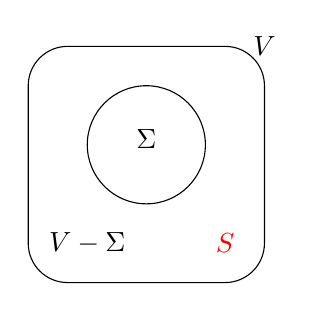
\begin{tikzpicture}
\draw [rounded corners=0.5cm] (-1,-1) rectangle ++(3,3) node [midway]{};

 \node at (0.5,0.82) (a) {$\Sigma$};
  \node at (-0.25,-0.5) (b) {$V-\Sigma$};
  \node at ( 1.5,-0.5) (c) {{\color{red}$S$}};
  \node at (2,2) (d) {$V$};
\draw (0.5,0.75) circle (0.75cm);
\end{tikzpicture}
\end{center}
A los elementos de $V-\Sigma$ se les llama \textit{símbolos no terminales}.
\subsubsection{Notación}
Para cada $A\in V-\Sigma \text{ , } w\in\Sigma^*$
$$
(A,w)\in R \Leftrightarrow A \xrightarrow[G]{} w
$$
Donde $G$ se refiere a la gramática.
\subsubsection{Derivación}
Para cada par de palabras $u,v \in V^*$ escribimos $u \xRightarrow[G]{} v$ ssi existen palabras $x,y,v' \in V^*,A\in(V-\Sigma)$ tales que:
$$
u = xAy ,\hspace{0.2cm} v = xv' y ,\hspace{0.2cm} A \xrightarrow[G]{} v'
$$
Se denota por $u \xRightarrow[G]{*} v$ la clausura reflexiva transitiva de $\xRightarrow[G]{}$
\subsubsection{Lenguaje Generado por $G$}
$$
L(G) = \Big\{ w\in \Sigma^* / S \xRightarrow[G]{*} w \Big\} 
$$
Un lenguaje es libre de contexto \textbf{ssi} existe una gramatica libre de contexto que genera el Lenguaje.
\subsection{Gramáticas Regulares}
\subsubsection{Definición}
Una Gramática Libre de Contexto $G=(V,\Sigma,R,S)$ es regular ssi:
$$
R \subseteq (V-\Sigma)\times \Sigma^*((V-\Sigma)\cup \{ \lambda \} )
$$
\subsubsection{Teorema}
Un lenguaje es Regular ssi es generada por una Gramática Regular:
\subsubsection*{Prueba}
\subsubsection*{ $\Rightarrow$}
Sea $M=(K,\Sigma,\sigma,s,F)$ construimos $G=(V,\Sigma , R,S)$ donde:
\begin{itemize}
\item $V= K \cup \Sigma$
\item $S = s$
\item $R = \{ q \rightarrow ap : \delta(p,a)=p \} \cup \{ q \rightarrow \lambda : q\in F \}$
\end{itemize}
\subsubsection*{$\Leftarrow$}
Sea $G = (V,\Sigma,R,S)$ construimos $M=(K,\Sigma,\Delta,s,F)$ donde:
\begin{itemize}
\item $K = (V-\Sigma) \cup \{f\}$ donde $f$ es un nuevo elemento.
\item $s=S$
\item $F=\{f\}$
\item $\Delta = \big\{ (A,w,B);A\rightarrow wB, A,B \in (V-\Sigma) ,w \in \Sigma^* \big\} \cup \big\{ (A,w,f);A\rightarrow w, A \in (V-\Sigma) ,w \in \Sigma^* \big\}$
\end{itemize}
\section{Autómata con Pila}
\subsubsection{Definición}
Un autómata con Pila es una sextupla:
$$
M = (K,\Sigma,\Gamma,\Delta,s,F)
$$
donde :
\begin{itemize}
\item $k:$ 
\item $\Sigma:$ Símbolos de Entrada
\item $\Gamma:$ es un conjunto finito no vacío \textit{(llamado alfabeto de la Pila).}
\item $s\in K$
\item $F \subseteq K$
\item $\Delta$ es un subconjunto finito de $(K\times\Sigma^*\times\Gamma^* ) \times (K\times\Gamma^*)$ (Relación de Transición)  
\end{itemize}
\subsubsection*{Significado de una Transición}
$$
((p,u,\beta),(q,\gamma)) \in \Delta
$$
\textit{''Estando en $p$ leyendo $w$ pasa al estado $q$ y reemplaza $\beta$ por $\gamma$.''}
\subsubsection*{Empujar a}
$$
((p,u,\lambda),(q,\alpha))\in\Delta
$$
\subsubsection*{Sacar de}
$$
((p,u,\alpha),(q,\lambda))\in\Delta
$$
\subsection{Configuración}
Una configuración es un elemento de:
$$
K\times\Sigma^* \times \Gamma^*
$$
\subsubsection*{La relación $\sststile{M}{\hspace{0.25cm}  \hspace{0.25cm}}$}
Para cada $((p,u,\beta),(q,\gamma))\in\Delta$ y para cada $x\in\Sigma^*, \alpha\in\Gamma^*$ definimos:
$$
(p,ux,\beta \alpha) \sststile{M}{\hspace{0.25cm} \hspace{0.25cm}} (q,x,\gamma\alpha)
$$
Para ilustrar un poco mejor la idea tenemos la siguiente gráfica:
\begin{center}
\begin{tikzpicture}[stack/.style={rectangle split, rectangle split parts=#1,draw, anchor=center}]
\node[stack=3] at (0,0) {
\nodepart{two}{$\beta$}
\nodepart{three}{$\alpha$}
};
\node at (1.5,0) (rel){$\sststile{M}{\hspace{0.25cm} \hspace{0.25cm}}$};
\node at (0,-1.25) (rel2){$(p,ux,\beta\alpha)$};
\node at (3,-1.25) (rel2){$(q,x,\gamma\alpha)$};
\node[stack=3] at (3,0) {
\nodepart{two}{$\gamma$}
\nodepart{three}{$\alpha$}
};
\node at (-0.75,1.5) (p){$p:$};
\node at (2.25,1.5) (q){$q:$};
\tikzstyle{bplus}=[rectangle split,rectangle split horizontal, rectangle split parts = 2, rectangle split empty part width=0.01mm, rectangle split every empty part={\hspace{0.25cm}}, draw]
\tikzstyle{every node}=[bplus]
\node at (0,1.5){u\nodepart{two}$x$};
\node at (3,1.5){\nodepart{two}$x$};
\end{tikzpicture}
\end{center}
\subsubsection*{Palabra aceptada por M}
Sea $w\in\Sigma^*$: \\ ${ }$ \\
$$
M \text{ acepta }w \Leftrightarrow (s,w,\lambda) \sststile{M}{\hspace{0.25cm} * \hspace{0.25cm}} (q,\lambda,\lambda) ; q\in F
$$
\subsubsection*{Lenguaje aceptado por M}
$$
L(M) =\{ w\in\Sigma^* / (s,w,\lambda) \sststile{M}{\hspace{0.25cm} * \hspace{0.25cm}} (q,\lambda,\lambda) ; q\in F \}
$$
\subsection{Autómatas con Pila y Gramáticas Libre de Contexto}
\subsubsection*{Definición}
La clase de lenguajes aceptados por autómatas con pila es exactamente la clase de lenguajes libres de contexto:
\subsubsection*{Prueba $\Leftarrow$}
Sea $G=(V,\Sigma,R,S)$ construimos $M=(K,\Sigma,\Gamma,\Delta,s,F)$ tal que $L(M)=L(G)$ donde:
$$
M = (\{p,q\},\Sigma,V,\Delta,p,\{ q\})
$$
\subsubsection*{Transiciones}
\begin{align}
((p,\lambda,\lambda),(q,S))&  \\
((q,\lambda,{\color{red}A}),(q,{\color{red}x}))&;\forall {\color{red}A}\rightarrow {\color{red}x} \in R \\
((q,{\color{red}a},{\color{red}a}),(q,\lambda))&;\forall {\color{red}a} \in \Sigma
\end{align}
\subsection{Propiedades de los Lenguajes Libres de Contexto}
\subsubsection*{Teorema}
Los lenguajes libres de contexto son cerrados bajo la unión, concatenación y estrella de Kleene.
\subsubsection*{Prueba}
Sean $G_i=(V_i,\Sigma_i,R_i,S_i)\hspace{0.5cm}i=1,2$ las Gramáticas Libres de Contexto y sin perdida de generalidad asumimos que $(V_1-\Sigma_1)$ y $(V_2-\Sigma_2)$ son disjuntos. 
\begin{itemize}
\item \subsubsection*{Unión}
$S$ es un nuevo símbolo
$$
G = (V_1\cup V_2 \cup \{ S\},\Sigma_1\cup\Sigma_2,R_1\cup R_2 \cup \{S\rightarrow S_1,S\rightarrow S_2 \},S )
$$
\item \subsubsection*{Concatenación}
$$
G=(V_1 \cup V_2 \cup \{ S\} ,\Sigma_1 \cup \Sigma_2,R_1 \cup R_2 \cup \{ S\rightarrow S_1 S_2 \},S )
$$
\item \subsubsection*{Estrella de Kleene}
$$
G = (V_1,\Sigma_1,R_1 \cup \{S_1\rightarrow\lambda, S_1 \rightarrow S_1 S_1 \} ,S_1)
$$
\end{itemize}
\subsubsection*{Teorema}
La intersección de un L.L.C con un lenguaje regular es un lenguaje libre de Contexto.
\subsubsection{Teorema de Pumping}
Sea $G$ una G.L.C. entonces existe un número $k$ que depende de $G$ tal que cualquier palabra $w\in L(G)$ de longitud $>k$, se puede reescribir $w=uvxyz$ de tal manera que ya sea $v$ o $y$ es no vacía y $uv^n xy^n z\in L(G)$. \textbf{Para cada} $n\geq 0$.
\subsubsection{Teorema}
Los L.L.C. no son cerrados bajo la complementación e intersección.
\section{Máquinas de Turing }
\subsubsection*{Definición}
Una máquina de Turing es una cuadrupla $M=(K,\Sigma,\delta,s)$ donde:
\begin{itemize}
\item $K:$ Conjunto Finito no Vacío , $h\notin K$
\item $\Sigma:$ Conjunto Finito no Vacío , $\#\in\Sigma , L,R\notin\Sigma$
\item $s\in K$
\item $\sigma: K\times\Sigma \rightarrow (K\cup\{h\}) \times (\Sigma\cup\{L,R\})$
\end{itemize}

\begin{enumerate}
\item {\color{red} Si $b\in\Sigma$ } la máquina reescribe $b$ por $a$.
\item {\color{red} Si $b=L$ } la cabeza lectora se mueve a la izquierda.
\item {\color{red} Si $b=R$ } la cabeza lectora se mueve a la derecha.
\end{enumerate}
\begin{center}
{\color{red}  Si la máquina esta en $h$} se dice que la máquina se \textit{detiene}.
\end{center}
\subsubsection{Interpretación}
\begin{center}
\begin{tikzpicture}

\draw(-5,5) -- (5,5);
\draw(-5,4) -- (5,4);

\draw [decorate, decoration={zigzag}] (5,5) -- (5,4);

\newcount\foo
\foo=-5
\loop
  \message{\the\foo}
  \draw(\foo,5) -- (\foo,4);
  \advance \foo 1
\ifnum \foo<5
\repeat

\node[] at (-4.5,4.5) 
    {b};
\node[] at (-3.5,4.5) 
    {b};
\node[] at (-2.5,4.5) 
    {a};
\node[] at (-1.5,4.5) 
    {a};
\node[] at (-0.5,4.5) 
    {b};
\node[] at (0.5,4.5) 
    {b};
\node[] at (1.5,4.5) 
    {\#};    
\node[] at (2.5,4.5) 
    {\#};
\node[] at (3.5,4.5) 
    {\#};
\node[] at (4.5,4.5) 
    {\#};


\draw[line width=0.4mm, red] (-1.1,3.9) -- (0.1,3.9) -- (0.1,5.1) -- (-1.1,5.1) -- (-1.1,3.9);

\draw[line width=0.2mm](-2,1) -- (2,1) -- (2,3) -- (-2,3) -- (-2,1);
\draw(-5,0.5) -- (5,0.5);

\draw[line width=0.2mm] (-1.5,0.75) circle (7pt);
\draw[line width=0.2mm] ( 1.5,0.75) circle (7pt);

\draw [->,very thick](2,2) -- (3,2);
\draw [->,very thick](-2,2) -- (-3,2);

\newcounter{cB} 

\newcommand\x{0}
\forLoop[45]{0}{7}
{%
  \node[] at ({sin(\i)*0.75},{cos(\i)*0.75+2}) {$q_{\thecB}$};
  \x = \the\numexpr\x+1 \relax;
  \addtocounter{cB}{1};
}
\node[] at ({sin(315)*0.75},{cos(315)*0.75+2}) {$h$};
\draw [->,very thick](0,2) -- ({sin(150)*0.5},{cos(150)*0.5+2});

\end{tikzpicture}
\\
En una Máquina de Turing la \textit{cinta} es infinita a la derecha.
\end{center}
\subsubsection*{Teorema}
Los siguientes modelos de máquinas de Turing son igualmente poderosos:
\begin{itemize}
\item La Máquina de Turing Estándar.
\item La Máquina de Turing de varias cabezas.
\item La Máquina de Turing de varias pistas.
\item La Máquina de Turing de varias cintas.
\item La Máquina de Turing Bidimensional.
\item Automata con Pila con 2 Pilas
\item IBM Mainframe
\end{itemize}